%%% Módulo 2:
%%  Camión tanque con emulsión. (C)
\item Un camión cisterna transporta en Brasil una mezcla de etanol-gasolina
con proporciones en volumen 50-50 \%. En principio ambas sustancias se encuentran
perfectamente mezcladas, pero luego de un tiempo de estar estacionada, la mezcla
se separa, como se muestra en la figura \ref{fig:tanque}.
El tanque se encuentra totalmente lleno, cerrado y presurizado de forma tal que
la presión mínima (punto \textbf{b}) es siempre 1 bar.
\\
Escriba las expresiones de la fuerza sobre la tapa trasera del tanque
para el caso de fases mezcladas y separadas para el caso estático y para el caso
en el que el camión acelera con aceleración $a_c$. Calcule también el torque
producido por la fuerza de hidrostática respecto del punto \textbf{a}.
\\
Una vez planteada la solución para un tanque prismático rectangular, modifíquela
para aplicarla a una cisterna cilíndrica de sección circular (más realista).
¿Pueden generalizarse estos resultados par cualquier proporción etanol-gasolina?

\begin{equation*}
\rho \qquad \vec{a}_c \qquad \vec{g} \qquad L \qquad H_0 \qquad B = H_0
\end{equation*}


\begin{figure}[h]
  \centering
  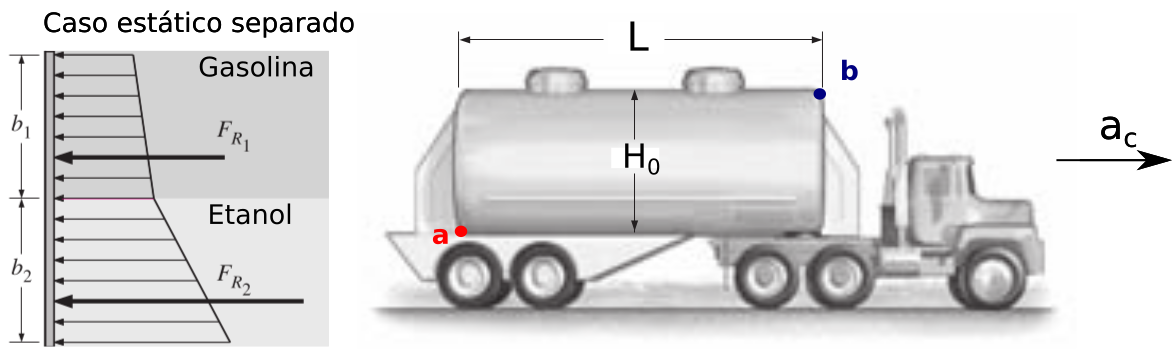
\includegraphics[width=0.9\textwidth]{camion.png}
  \caption{Camión cisterna con detalle de separación de fases (no está a escala)}
  \label{fig:tanque}
\end{figure}



